\section{Level 1 Decompositions}
\label{sec:level-1}

\npar In the first level, the whole system, ReMeS is decomposed. 

\subsection{ReMeS (Whole System)}
\label{dec:whole-system}

\npar In the first step of the ADD process, the whole system is decomposed in
two subsystems ``Remote Module Subsystem'' and ``Portal''. The decomposition is
shown in figure \ref{fig:dec/level-1}.

\begin{figure}[H]
	\begin{centering}
		% TODO
		%\includegraphics[width=0.6\textwidth]{figs/decomposition/whole-system/decomposition.pdf}
		\caption{The level 1 decomposition of the ReMeS system}
		\label{fig:dec/level-1}
	\end{centering}
\end{figure}

\subsubsection{Architectural Drivers}
\label{drivers:whole-system}

\npar For the first decomposition, two high priority quality attribute scenarios
and their associated use cases are taken into account. 

\begin{itemize}
 	\item Av1 (High): Measurement database Failure
 	\begin{itemize}
 		\item UC8 (High): Send measurement
 		\item UC13 (High): Send alarm 
 	\end{itemize}
  	\item P1 (High): Timely closure of valves
  	\begin{itemize}
  		\item UC13 (High): Send alarm 
		\item UC11 (Medium): Operate actuator remotely 
  	\end{itemize}
\end{itemize}

\npar The considered use cases includes the use cases listed below. 

\begin{itemize}
	\item UC7 (High): Send trame to remote device
	\item UC9 (High): Notify customer
	\item UC10 (Medium): Detect anomaly
\end{itemize}

\npar Based on the architectural drivers, the remote module subsystem has to
provide functionality for remote module communication (receiving and sending
trames), trame storage, trame processing and customer communication. 

\npar In order to obtain a better understanding of the relationships between
these functionalities, a small domain model is drafted. Figure
\ref{fig:dec/whole-system/draft} This model can then be refined later on
in this level of decomposition.

\begin{figure}[H]
	\begin{centering}
		% TODO
		%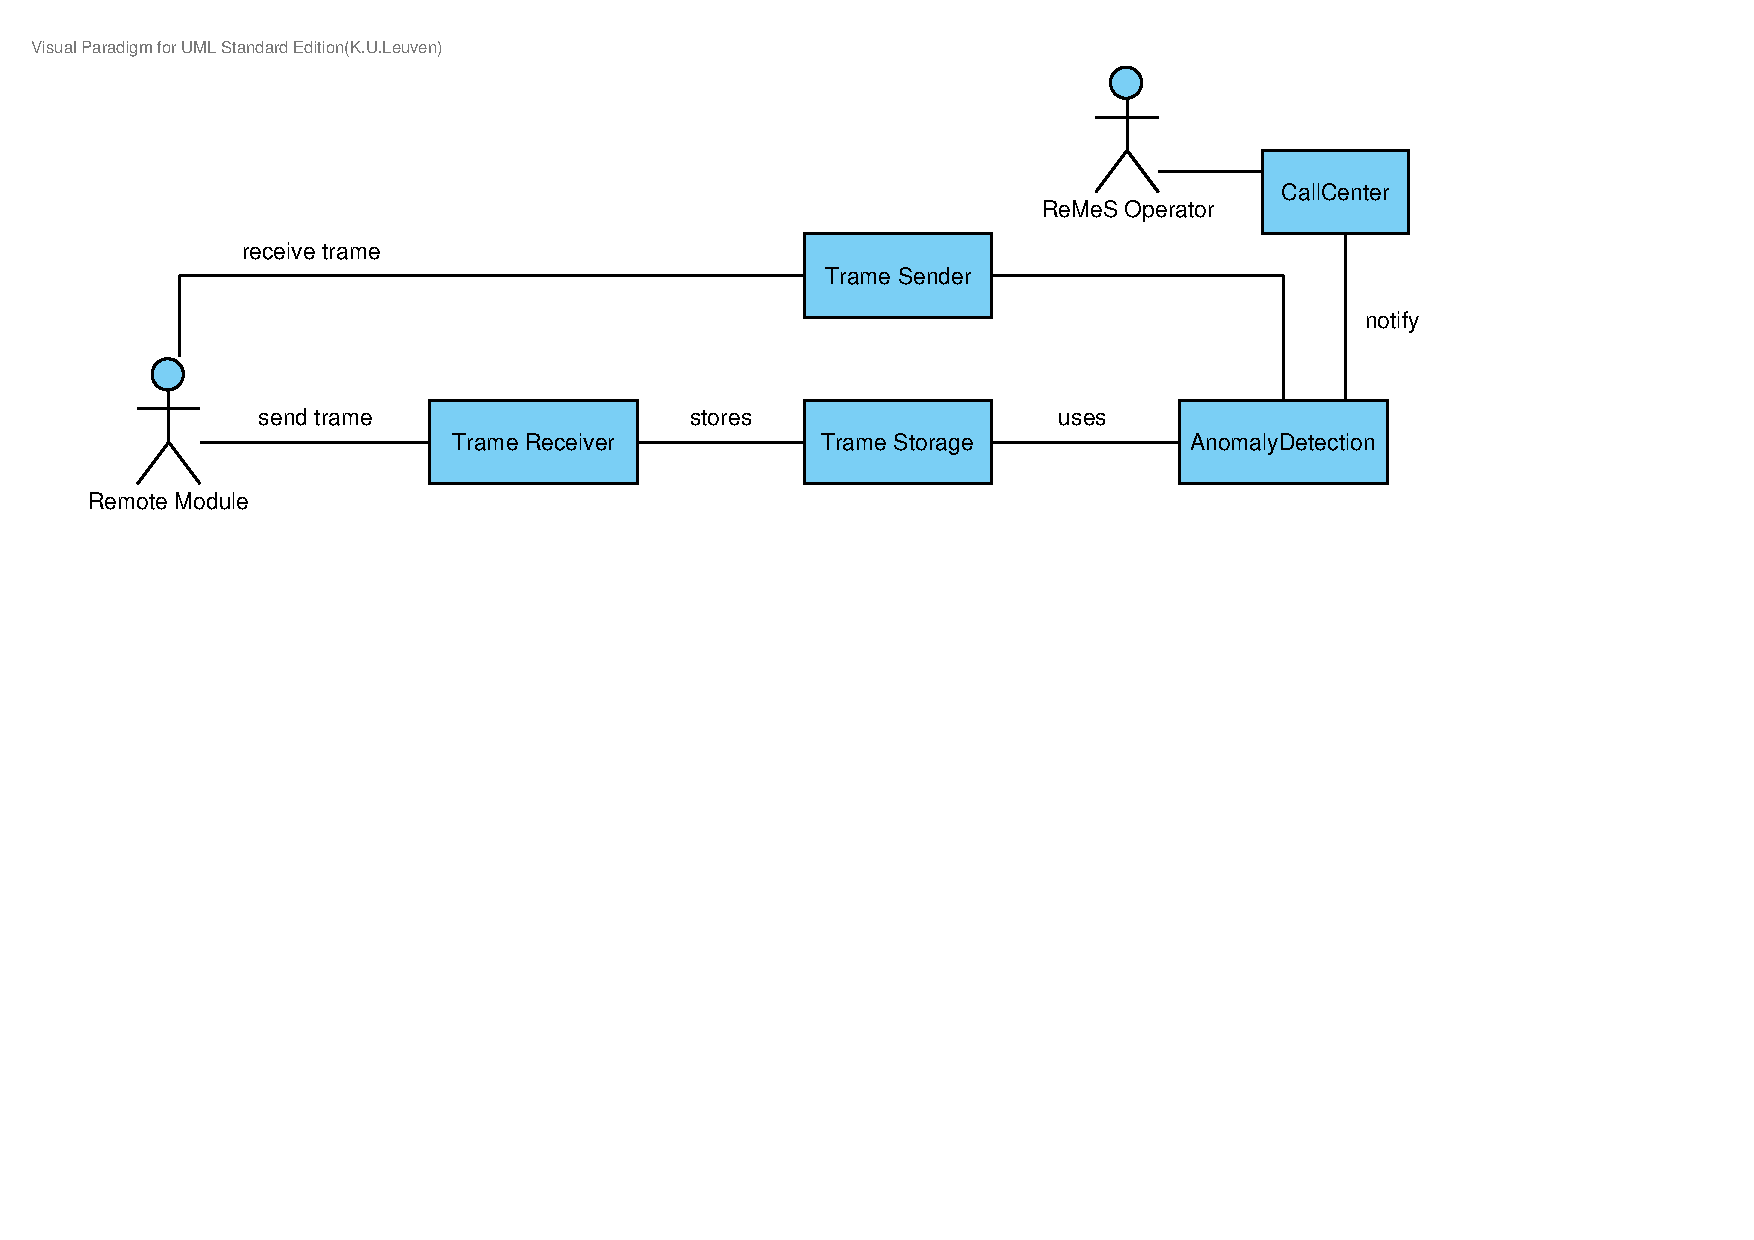
\includegraphics[width=0.6\textwidth]{figs/decomposition/whole-system/domainmodel-draft.pdf}
		\caption{Draft of the domain model used in the level 1 decomposition}
		\label{fig:dec/whole-system/draft}
	\end{centering}
\end{figure}

\subsubsection{Tactics}
\label{tactics:whole-system}

\paragraph{Availability}

\npar After selecting the drivers for the current decomposition, one has to
choose the tactics to achieve them. Recall from section
\ref{drivers:whole-system} that the first driver was Av1. All approaches to
maintain availability involve either detection, recovery or prevention of
faults.

\npar First of all, a fault needs to be detected. For this, there are three
options: ping/echo, heartbeat and exceptions. It is important to notice that the
latter is not very practical. This can be illustrated with a simple example.

\npar Suppose that a component $c_1$ depends on another component $c_2$. For
some reason, $c_1$ does not need the services of $c_2$ for a duration longer
than the detection interval of 5 seconds (see Av1). Within this time, no
detection can occur, simply because there is no interaction between the
components. For this reason, we eliminate exceptions as a primary fault
detection system. However, exceptions will still have to be implemented in order
to make the system fail gracefully (a component being unavailable will not
cause the system to crash).

\npar Another detection method uses ping/echo. This primarily focusses on
network connectivity and will not check the availabillity of the service itself.
Again, this is not very practical. A server can be reachable, but the service on
a certain port number may be unavailable. In this case, the ping/echo
method would not detect the fault. 

\npar Heartbeat on the other hand, will be part of the system itself and will be
able to check whether the service is still up and running. It will periodically
(at most every 5 seconds) check the state of the system and send out a pulse
to a heartbeat monitor if everything is runnning fine.

\npar Another advantage of using heartbeat is that the pulse can contain data,
more specifically status data. For instance, a single failing disk in a RAID5
array can cause a warning but will not cause the system to crash. This
information can be included in the pulse of the heartbeat to inform the
administrators to replace the failing disk.

\npar As a result, heartbeat seems the best solution to detect faults. 

\npar Detecting a fault is insufficient, resolving the fault is at least equally
important. Once a fault has been detected, the faulting component must be taken
out of action and be repaired or replaced with a working version. However, in
order to guarantee an uptime of 99.9\%, there has to be a backup to take over in
case of a component fault.

\npar As was the case in the previous paragraph, there are many alternatives.
The most frequently used ones are active redundancy, passive redundancy and
spare. The main criterion to select one of these is the downtime of the system.
These downtimes are respectively in the order of miliseconds, seconds and
minutes. An uptime of 99.9\% corresponds to 0.72 hours (= 43.2 minutes) of
permitted downtime on a monthly basis. This number reveals potential problems
when a spare is used because there can be only less the 10 failures a month. For
this reason, use of spares is eliminated.

\npar The difference between active and passive replication is rather subtle.
In an active replication scheme, the system will recover faster then in a
passive replication scheme. However, all replicas should be in a consistent
state. This increases the communication overhead, compared to a passive
replication scheme. 

\npar On the other hand, the active replication scheme can also provide load
balancing. If one replica has a higher load than another, the replica with the
lowest load can be used to process the query. For this reason, the active
replication scheme is selected. 

\paragraph{Performance} 

\npar For performance tactics there are three categories: resource
arbitration, resource management and resource demand.

\npar If there is more than one request to gain control over a resource, there
has to be some form of scheduling. By far the most used one is a priority
scheduler where request are served earlier when they have a higher priority.
This is particulary useful for alarms to still reach the appropriate parties in
time even when the system is in overload mode. 

\npar Secondly there is resource management. To process more than one trame at a
time, concurrency can be introduced. This can be done in various ways. Several
threads can be started on one processor, on separate processors or even on
separate systems. Another possibilitiy is off course increasing the available
hardware but since this is not a very cost effective solution, this is left out
of consideration.

\npar On a lower level one could also try to minimize network overhead by
only sending small amounts of data in each trame. This is achieved by
limiting the size of the trames to 160 bytes.

\npar To conclude a small overview is given of all selected tactics for this
decomposition.

\begin{itemize}
 	\item Av1 (High): Measurement database Failure
 	\begin{itemize}
 		\item Detection: Heartbeat 
 		\item Recovery : Active replication
 	\end{itemize}
  	\item P1 (High): Timely closure of valves
  	\begin{itemize}
  		\item Resource arbitration : Scheduling
		\item Resource management  : concurrency
		\item Resource demand      : limited tramesize
  	\end{itemize}
\end{itemize}

\subsubsection{Design Patterns}
\label{dp:whole-system} %TODO verder uitwerken

\npar With respect to resource arbitration and resouce management, the
\emph{Active Object} design pattern is chosen for trame communication and
processing. Schedulers will determine the order in which trames are received,
processed and sent. These schedulers will have different scheduling policies,
implemented with the \emph{Strategy} design pattern, in order to allow operation
in different modes.

\npar The trames will have to be objectified. This will yield two advantages.
Firstly, the scheduler can be implemented using the \emph{Command Processor}
design pattern. Secondly, a unified language will exist for all vendor
specific trame formats.

\npar To make the data highly available, the database will be replicated. This
can be achieved by using the \emph{Replicated Component Group} design pattern.
The database will be replaced with a front-end interface that replicates all
requests to all the replicas. 

\subsubsection{Other requirements}
\label{others:whole-system}





